% !TEX encoding = UTF-8 Unicode
\documentclass[10pt,ngerman]{scrartcl}
\usepackage{url,bm,tikz,a4wide}
\usepackage[utf8]{inputenc}
\usepackage{booktabs}
\usepackage{amsmath,amssymb}
\usepackage[english]{babel}
\usepackage{graphicx,tikzsymbols} 
\usepackage{xcolor}
\usepackage[numbers]{natbib}
\usepackage{float}
\usepackage{gensymb}

\DeclareOldFontCommand{\bf}{\normalfont\bfseries}{\mathbf}

\usepackage{nicefrac,xfrac}

\renewcommand{\theenumi}{\alph{enumi})}
\renewcommand{\theenumii}{\Roman{enumii}}

\setcounter{secnumdepth}{-1}

\begin{document}

\begin{figure}[htbp]
\begin{minipage}[b]{0.50\linewidth}
\begin{Large}
	\textbf{Group Number:} 2\\
	\\
	
\end{Large}
\end{minipage}
\begin{minipage}[b]{0.50\linewidth}
\begin{flushright}
\begin{Huge}
\textbf{Physics}\\
\end{Huge}
\vspace{0.5cm}
\begin{large}
Winter term 2021/22
\end{large}
\end{flushright}
\end{minipage}
\end{figure}

\vspace{2cm}
\begin{huge}
\noindent

\textbf{Group Work}
\end{huge}

\section{1 Momentum and Force. Fields of Force}
\subsection{1.1 Momentum and Force. Fields of Force}
The so-called neutron stars have about the mass of our sun (ca. $2 \cdot 10^{30}kg$) and a typical diameter of about 20 km. Their mean mass density is roughly that of an atomic nucleus.
\begin{enumerate}
	\item How big is the mean mass density?
	\item According to Newton's law of gravitation, how heavy would a piece of weight with the mass of 1kg be on the surface of a neutron star?
	\item How heavy would $1mm^3$ of neutron star matter be on earth and what diameter would an iron ball of the same mass have?
\end{enumerate}

\subsection{1.2 Coulomb interaction of two electrons}
Sketch correctly to scale the course of the magnitude of the force with which two electrons repel each other at distances of $0,5 \cdot 10^{-10}$m to $5,0 \cdot 10^{-10}$m according to Coulomb's law.

\newpage
\section{2 Work and Power. Energy. Heat and Temperature}
\section{2.1 train set}
For example, the electric drive of a train set consumes the power shown in the figure below during a operational cycle (1 MW = 106 W).

\begin{enumerate}
	\item What is the total electrical energy consumed during this operational cycle?\\\\
	$
	\begin{array}{l}
		P_{1} \ =\ \frac{7MW\cdot \ 120s}{2} \ =\ 420\ MWs\ =\ 420\ MJ\\
		P_{2} \ =\ 2\ MW\ *\ 600s\ =\ 1200\ MW\ =\ 1.2\ GJ\\
		P_{3} \ =\ \frac{-7MW\ *\ 60s}{2} \ =\ -240\ MW\\
		P_{total} \ =\ P_{1} \ +\ P_{2} \ +\ P_{3} \ =\ 420\ MJ\ +\ 1.2\ GJ\ -\ 240\ MJ\ =\ 1.38\ GJ
		\end{array}
	$
	\item What is the mean power consumed?\\\\
	$
        P_{mean} \ =\ \frac{P_{total}}{\Delta t} = \frac{1.38\ GJ}{\Delta t_{1} +\Delta t_{2} +\Delta t_{3} +\Delta t_{4}} \ =\ \frac{1.38\ GWs}{120s\ +\ 600s\ +\ 60s\ +\ 60s} \ =\ 1.643\ MW
    $
\end{enumerate}

\begin{figure}[H]
	\centering
	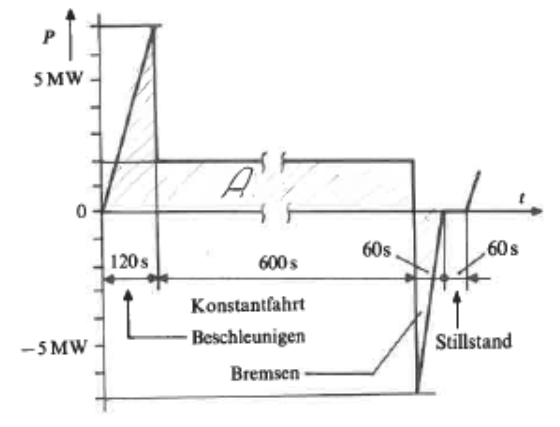
\includegraphics[scale=0.5]{group_work_1.png}
\end{figure}

\section{2.2 crash test facility}
In a crash test facility, a vehicle including cuts m = 900 kg is accelerated uniformly via an electric linear motor through a distance s = 20 m with a constant force F = 5 kN.
\begin{enumerate}
	\item How big is the necessary electrical energy in kWh if all losses are neglected?
	\item How big is the final speed achieved? During the subsequent impact process, the vehicle is brought to a standstill within a distance of s = 80 cm.
	\item What is the mean force that acts on a fictitious seated occupant, m1 = 80 kg?
\end{enumerate}

\section{2.3 Connected load of a flow heater}
Suppose you want to design an electric water heater without a storage tank that heats a water flow of 0,1 l/s from 10 °C to 60 °C. What is the minimum required electrical connection power? (specific heat capacity of water c = 4,19 kJ/(kgK)).

$
\begin{array}{l}
T_{in} = 10\degree C\\
T_{out} = 60\degree C\\
\Delta T=50^{\degree } C\ =\ 50K\\
water\ flow\ =\ 0.1\ l/s\\
m\ =\ 0.1 kg\\
specific\ heat\ capacity\ of\ water\ c\ =\ 4.19kJ/( kgK)\\
total\ energy\ to\ heat\ up\ 0.1 l\ water\ \Delta Q\ =\ c\ *\ m\ *\ \Delta T\\
minimum\ required\ electrical\ connection\ power\ [ W] \ =\ kWh\\
\\
Required\ energy\ to\ heat\ up\ 0.1\ kg\ water\ from\ 10\degree C\ to\ 60\degree C\\
\left[\Delta Q\right] \ =\ K\ *\ kg\ *\ \frac{kJ}{kg\ *\ K} \ =\ kJ\\
\Delta Q\ =\ 50\ *\ 0.1\ *\ 4.19\ =\ 20.95\ kJ\\
\\
Required\ connection\ power\ to\ heat\ up\ 0.1l/s\ water\ from\ 10\degree C\ to\ 60\degree C\\
\left[ P\right] \ =\ W\\
P = 1000\ *\ kJ\ \ /\ t_{s} \ ( we\ need\ this\ energy\ every\ second\ to\ heat\ up\ the\ water\ constantly)\\
P\ =\ 1000\ *\ 20.95\ /\ 1\ =\ 20950W\ =\ 20.95kW

\end{array}
$

\end{document}